\chapter[Escopo]{Escopo}

Esta seção apresenta o contexto no qual a melhoria será aplicada explicitando o software e suas funcionalidades, os objetivos e premissas do projeto.

\section{Contexto}

No semestre 2016.1 na UnB, foi desenvolvido um projeto de \textit{software} com o nome \textbf{FarmManager}, na disciplina de Desenho de \textit{Software}. Este projeto tinha como principal finalidade a gestão operacional e financeira de uma fazenda de criação de gado e produção de leite no Estado de Goiás.

O FarmManager se encontra concluído, e apresenta extensa documentação, que pode ser encontrada em um repositório do \textit{Github}, ferramenta \textit{web} para controle de versão. A motivação para o uso deste projeto é, principalmente, o fato de embora apresentar qualidade, não ter tido a oportunidade de ser implantado. Isso ocorreu principalmente pelo fato do time que o desenvolveu focar em outros aspectos, como desenvolvimento de novas funcionalidades, maior documentação, dentre outros.

\subsection{Repositório do Github}

O projeto FarmManager foi desenvolvido por uma equipe com o auxílio do \textit{Github} para maior colaboração e organização.

O link do respositório é \url{https://github.com/EduardoMoreira/Desenho-UnB-2016-01}.



\section{Cronograma}

\begin{figure}[h!]
	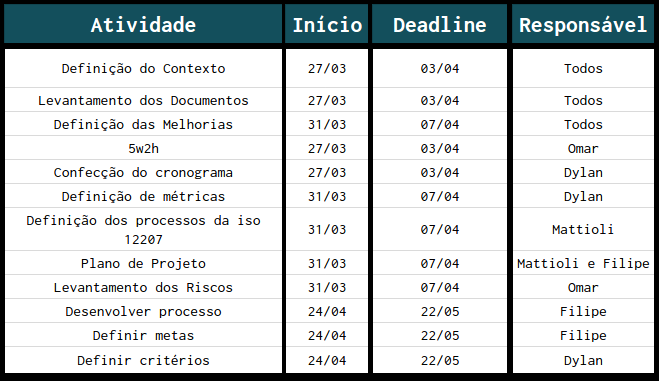
\includegraphics[keepaspectratio=true,scale= 0.65]{figuras/cronograma-mps.png}
	\caption{Cronograma}
	\label{eap}
\end{figure}

\subsection{Recursos}

Esta seção tem como objetivo definir os recursos humanos, materiais e de infra-estrutura necessários para a execução deste projeto.

Os recursos materiais e de infra-estrutura são de posse dos membros da equipe e também são usados em outros projetos. Não há necessidade, desta forma, de qualquer aquisição. 

\begin{table}[h!]
\centering
\caption{Papéis da Equipe}
\label{papeisDaEquipe}
\begin{tabular}{|l|l|}
\hline
\multicolumn{1}{|c|}{\textbf{Membro}} & \multicolumn{1}{c|}{\textbf{Função}}              \\ \hline
João Paulo                            & Líder                                             \\ \hline
Ebenezer                              & Gerente                                           \\ \hline
Heleno                                & Sub-Gerente (Projeto Eletrônico)                  \\ \hline
Mateus                                & Sub-Gerente (Projeto de Software)                 \\ \hline
Renata                                & Sub-Gerente (Projeto de Energia)                  \\ \hline
Pedro                                 & Sub-Gerente (Projeto de Automotiva e Estrutura)   \\ \hline
Bruno                                 & Desenvolvedor (Projeto Eletronico)                \\ \hline
Ricardo                               & Desenvolvedor (Projeto Eletronico)                \\ \hline
Omar                                  & Desenvolvedor (Projeto Software)                  \\ \hline
Maxwell                               & Desenvolvedor (Projeto Software)                  \\ \hline
Rita                                  & Desenvolvedora (Projeto de Energia)               \\ \hline
Luís                                  & Desenvolvedor (Projeto de Energia)                \\ \hline
Leonardo                              & Desenvolvedor (Projeto de Automotiva e Estrutura) \\ \hline
Arthur                                & Desenvolvedor (Projeto de Automotiva e Estrutura) \\ \hline
\end{tabular}
\end{table}

\begin{table}[h!]
\centering
\caption{Atividades e Responsáveis}
\label{atividadeseResponsaveis}
\begin{tabular}{|l|l|l|}
\hline
Tipo de Atividade  & Atividade                            & Responsável                      \\ \hline
Concepção          & Projeto Eletrônico                   & Heleno, Bruno e Ricardo          \\ \hline
Pesquisa e Escrita & Sistema de Aquisição de Dados        & Heleno                           \\ \hline
Pesquisa e Escrita & Placa de Condicionamento             & Bruno                            \\ \hline
Pesquisa e Escrita & Sistema de Controle                  & Bruno                            \\ \hline
Pesquisa e Escrita & Protocolo de Comunicação             & Ricardo                          \\ \hline
Pesquisa e Escrita & Sensores                             & Heleno, Bruno, Pedro e Ricardo   \\ \hline
Pesquisa e Escrita & Sistema de Arrefecimento             & Arthur e Rita                    \\ \hline
Pesquisa e Escrita & Sistema de Lubrificação              & Arthur                           \\ \hline
Pesquisa e Escrita & Sistema de Exaustão                  & Arthur                           \\ \hline
Modelagem          & Layout do Laboratório                & Pedro, Leonardo                  \\ \hline
Modelagem          & Sistema estrutural                   & Leonardo e Pedro                 \\ \hline
Pesquisa e Escrita & Sistema de Ignição                   & João Paulo                       \\ \hline
Pesquisa e Escrita & Análise do motor                     & Leonardo, Pedro                  \\ \hline
Pesquisa e Escrita & Sistema de Admissão                  & Luis                             \\ \hline
Pesquisa e Escrita & Sistema de Instalação do Dinamômetro & Renata                           \\ \hline
Pesquisa e Escrita & Análise de Testes                    & Renata                           \\ \hline
Pesquisa e Escrita & Documento de Visão                   & Ebenezer, Maxwell, Omar e Mateus \\ \hline
Modelagem          & Diagrama de Arquitetura              & Ebenezer e Mateus                \\ \hline
Modelagem          & Diagrama de Caso de Uso              & Omar e Maxwell                   \\ \hline
Pesquisa e Escrita & Documento de Arquitetura             & Ebenezer, Maxwell, Omar e Mateus \\ \hline
Modelagem          & Estruta Análita do Projeto           & Todos os autores                 \\ \hline
Modelagem          & Cronograma                           & Ebenezer                         \\ \hline
\end{tabular}
\end{table}

\subsection{Riscos}

\begin{landscape}
% Please add the following required packages to your document preamble:
% \usepackage[table,xcdraw]{xcolor}
% If you use beamer only pass "xcolor=table" option, i.e. \documentclass[xcolor=table]{beamer}
\begin{table}[]
\centering
\caption{Tabela de Riscos do Projeto}
\label{tabela-de-riscos}
\begin{tabular}{|l|l|c|c|c|l|l|}
\hline
\rowcolor[HTML]{EFEFEF} 
\textbf{\#} & \textbf{Riscos}                                                                                                                 & \textbf{Probabilidade} & \textbf{Impacto}                   & \textbf{Prioridade} & \multicolumn{1}{c|}{\cellcolor[HTML]{EFEFEF}\textbf{Ação de Mitigação}}                                                                  & \multicolumn{1}{c|}{\cellcolor[HTML]{EFEFEF}\textbf{Ação de Contingência}}                                                      \\ \hline
1           & \begin{tabular}[c]{@{}l@{}}Atraso na entrega\\ das atividades\end{tabular}                                                      & Média                  & \cellcolor[HTML]{FFFC9E}Médio      & 5                   & \begin{tabular}[c]{@{}l@{}}Cobrança interna entre\\ os integrantes do grupo\end{tabular}                                                 & \begin{tabular}[c]{@{}l@{}}Priorizar essas atividades afim\\ de diminuir o impacto do atraso\end{tabular}                       \\ \hline
2           & \begin{tabular}[c]{@{}l@{}}Não adoção da\\ melhoria pelo\\ grupo\end{tabular}                                                   & Baixa                  & \cellcolor[HTML]{FFCE93}Grave      & 3                   & \begin{tabular}[c]{@{}l@{}}Elaborar plano de melhoria\\ claro e de concordância de\\ todo o grupo\end{tabular}                           & \begin{tabular}[c]{@{}l@{}}Realizar aprimoramento do\\ plano de melhoria através de\\ consulta à literatura\end{tabular}        \\ \hline
3           & \begin{tabular}[c]{@{}l@{}}Estimativas\\ equivocadas\end{tabular}                                                               & Alta                   & \cellcolor[HTML]{FFFC9E}Médio      & 4                   & \begin{tabular}[c]{@{}l@{}}Consultar e obter experiências\\ de alunos e professores com\\ maior conhecimento na área\end{tabular}        & \begin{tabular}[c]{@{}l@{}}Alteração das estimativas e\\ planejamento\end{tabular}                                              \\ \hline
4           & \begin{tabular}[c]{@{}l@{}}Falta de\\ comprometimento\\ ou de motivação\\ por parte dos\\ integrantes\end{tabular}              & Baixa                  & \cellcolor[HTML]{FFFC9E}Médio      & 7                   & \begin{tabular}[c]{@{}l@{}}Realizar dinâmicas para inserir\\ os integrantes no processo\\ aumentando a atuação dos\\ mesmos\end{tabular} & \begin{tabular}[c]{@{}l@{}}Realizar pareamento com o\\ integrante desmotivado afim\\ de dar maior auxílio ao mesmo\end{tabular} \\ \hline
5           & \begin{tabular}[c]{@{}l@{}}Falta de\\ conhecimento\\ técnico ou\\ gerencial dos\\ integrantes sobre\\ os processos\end{tabular} & Alta                   & \cellcolor[HTML]{FFCCC9}Gravíssimo & 1                   & \begin{tabular}[c]{@{}l@{}}Realizar estudos e pesquisas\\ para aprimorar o conhecimento\\ da equipe\end{tabular}                         & \begin{tabular}[c]{@{}l@{}}Realizar consulta com o\\ professor para sanar dúvidas\end{tabular}                                  \\ \hline
6           & \begin{tabular}[c]{@{}l@{}}Desistência de\\ um ou mais\\ integrantes\\ do grupo\end{tabular}                                    & Baixa                  & \cellcolor[HTML]{FFCCC9}Gravíssimo & 2                   & \begin{tabular}[c]{@{}l@{}}Priorizar atividades em pares\\ afim de haver maior interação\\ entre os integrantes\end{tabular}             & Reorganização da equipe                                                                                                         \\ \hline
\end{tabular}
\end{table}
\end{landscape}

\subsubsection{Legenda}

\textbf{Risco leve}: Risco que praticamente não impactará o andamento normal do projeto.

\textbf{Risco médio}: Risco que impactará levemente o andamento do projeto.

\textbf{Risco grave}: Risco que impactará o andamento do projeto, porém não impedirá o andamento do mesmo.

\textbf{Risco gravíssimo}: Risco que impedirá o andamento do projeto.